
\section{Motivation}


The toric code is the simplest and most elegant of the class of topological codes \cite{topological_codes}. The code uses $2n^2$ physical qubits to encode two logical qubits. The code's properties are usually studied in the large-$n$ limit, where it has been shown that the ideal code can protect against errors on $18.9\%$ of the phsyical qubits \cite{bombin12}. In practice the threshold obtained depends not only on the code, but also on the decoding algorithm used. The search for an efficient, high-threshold decoding alogithm has attracted a lot of attention recently, and there are a number of decoders that approach the theoretical threshold \cite{wooton_mcmc1, poulin_renormalisation, poulin_renormalisation2} [TODO need a reference for best threshold using Edmonds type approach].

When the operations required to perform the code are taken into account, the error rates tolerated fall to $0.75\% - 1.4\%$ depending on the error model \cite{raussendorf07, fowler11, ghosh_fowler}, which seems less impressive when compared with tolerated error rates of $3.2\%$ \cite{?Knill} demonstrated for concatenated codes. The advantage of the toric and other stabiliser codes is that only local operations are required, making a scalable physical implementation more realistic.


\section{Review of the Toric Code}

\subsection{Defining the Code}



Joint eigenstate - dimension - one way to get there is by measurement




\subsection{Detecting Errors}



Depends on the error model.


It is worth noting that it is not necessary to physically perform the matching operation on the physical qubits; as a Pauli operation on a given qubit can just be considered a redefinition of the local basis, it is enough to keep track of the operations that would be performed at each stage, provided these are taken into account on any further operations that are performed.


\section{Decoders}




\section{error models}

In the rest of the paper we assume that we start in a known initial state, corresponding to the zero-syndrome and known logical states. In the experimental procedure described above this is not the case, as our initial stabilisers may have mis-reported. Thankfully in the decoding step (\ref{decode_step}) we are concerned only with the difference between the initial and final sydromes, and so the two situations are equivalent albeit with a modified mis-reporting probability $q$. In order to interpret the results given later we must set $q = 2q_\text{expt}(1-q_\text{expt})$, where $q_\text{expt}$ is the actual stabiliser measurement mis-reporting probability for the system. An improved experimental procedure would involve aborting any experiment where an odd number of stabilisers fire in the initial measurement, which would make initialisation mis-reports an $O(q_\text{expt}^2)$ event and allow $q \approx q_\text{expt}$ for small $q_\text{expt}$.

\section{decoders}
\section{Precomputed decoder}

\section{Single channel noise}

We first envisage a system where there is a single dominant error channel. Without loss of generality we take this to be the $Y$ channel, setting $p_y = p$ and $p_x = p_z = 0$ in equation (\ref{noise_eq}). In this choice we optimize the code against the given dominant error: $Y$ errors are detected in both the $X$ and $Z$ syndromes, giving us the most information to work with during the decoding step.

\begin{figure}[htb]
  \begin{center}
    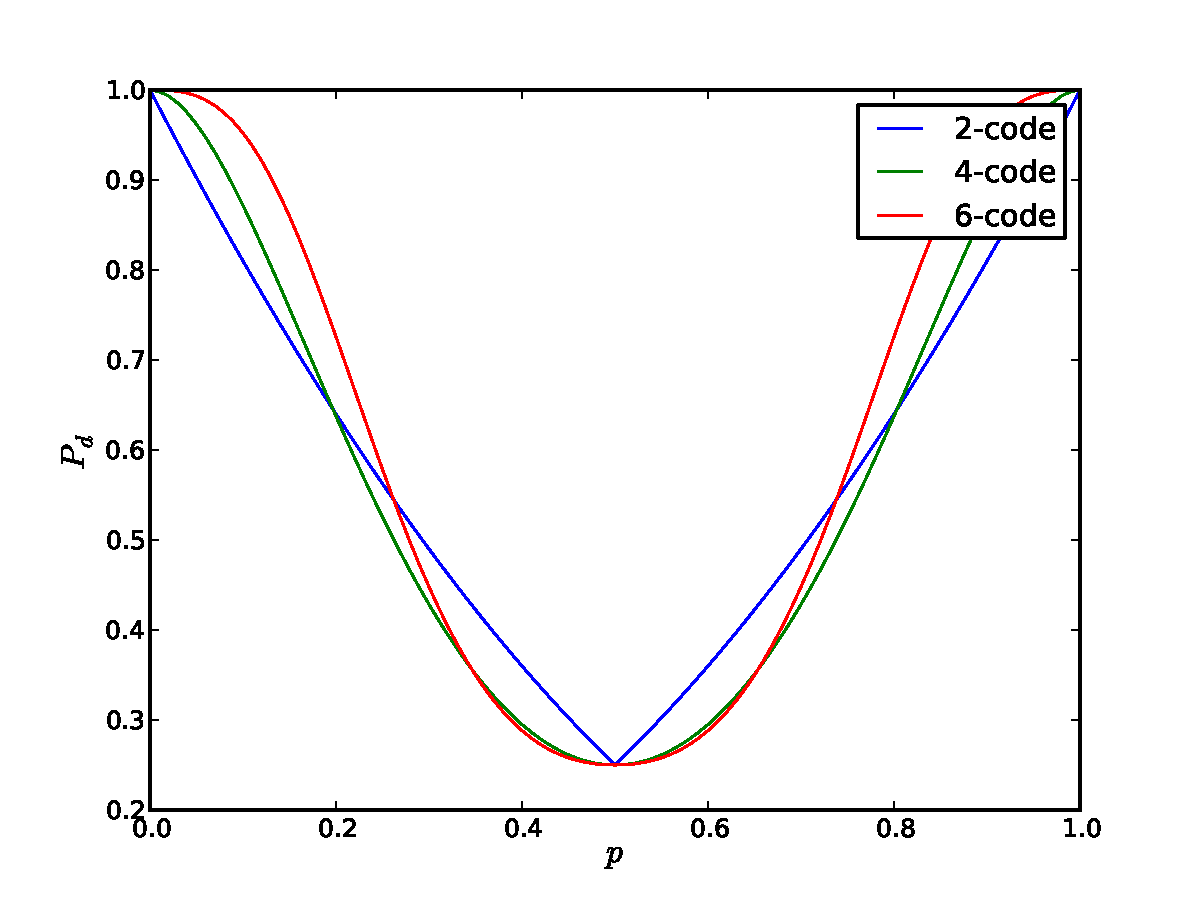
\includegraphics[width=8cm]{assets/y_truthful.pdf}
  \end{center}
  \caption{Success probabilities for toric code on a grid that suffers only from y errors. We use x- and  z-stabiliser information to correct y-errors, in order to recover the x or z components of the encoded qubits.}
  \label{y_truthful}
\end{figure}

We find that the first non-trivial code, the $4$-code, offers encoding power in this scenario (Fig. \ref{y_truthful}). The $4$-code has both error-detect and error-correct capability and outperforms the $2$-code up to a physical qubit error probability of around $20\%$. It is worth contrasting this with the $4$-code protecting against single channel $X$ noise, which offers no error-correct capabilities: even a single isolated error has a decoding probability of at most $0.5$, as there are always two equally likely matchings (see Fig. \ref{4-code_error_correct}).

\begin{figure}[htb]
  \begin{center}
    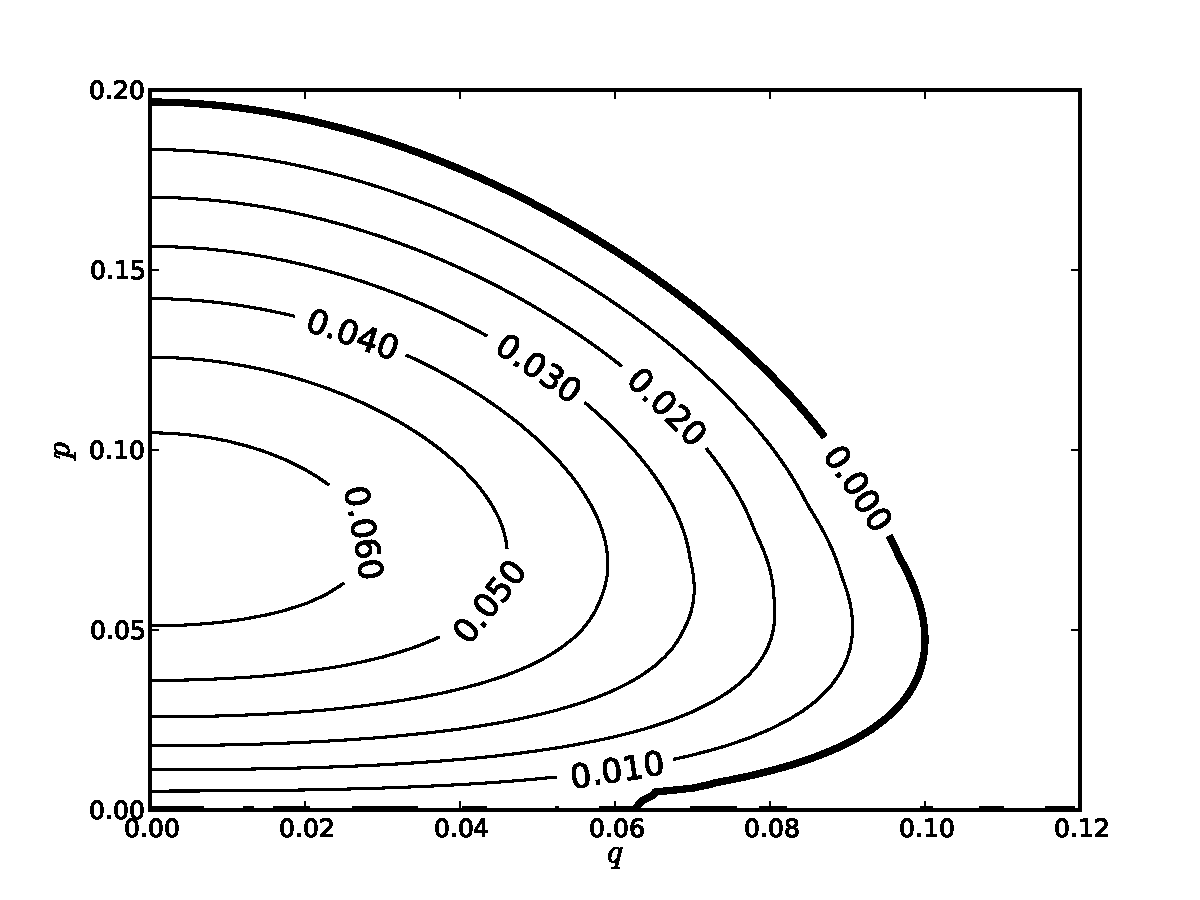
\includegraphics[width=8cm]{assets/y_lying.pdf}
  \end{center}
  \caption{Decoding success probabilities for the full quantum $6$-code with mis-reported stabiliser outcomes.}
  \label{y_lying}
\end{figure}

When protecting against single channel $Y$ noise, the $4$-code shows remarkable resilience against stabiliser outcome mis-reports, being able to comfortably deal with mis-reporting probabilities in the region of $5\%$ (Fig. \ref{y_lying}).

\section{Full channel noise}

We now look at the full depolarizing noise model, taking $p_x = p_y = p_z$ in equation (\ref{noise_eq}). 

\begin{figure}[htb]
  \begin{center}
    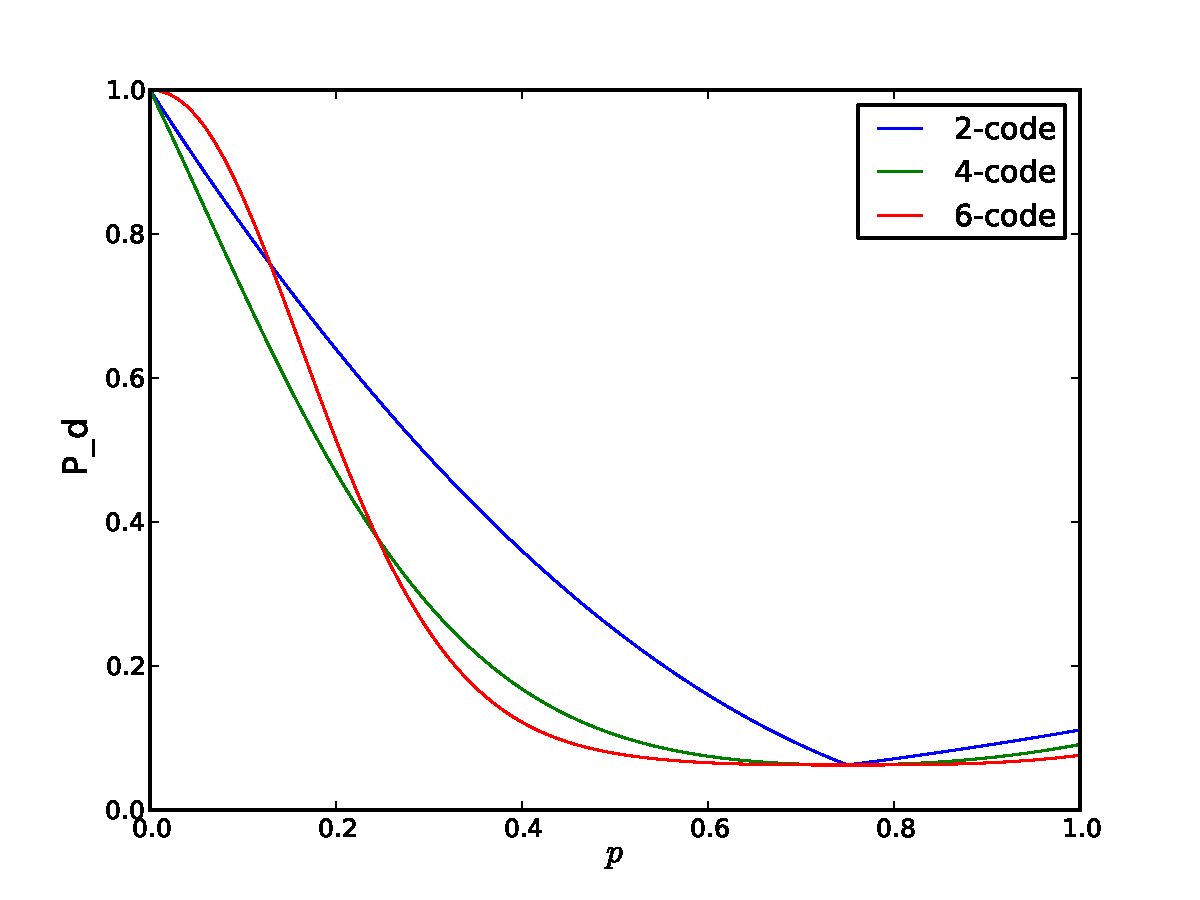
\includegraphics[width=8cm]{assets/full_truthful.pdf}
  \end{center}
  \caption{Success probabilities for full toric code with perfect stabiliser outcome reporting.}
  \label{full_truthful}
\end{figure}
\begin{figure}[htb]
  \begin{center}
    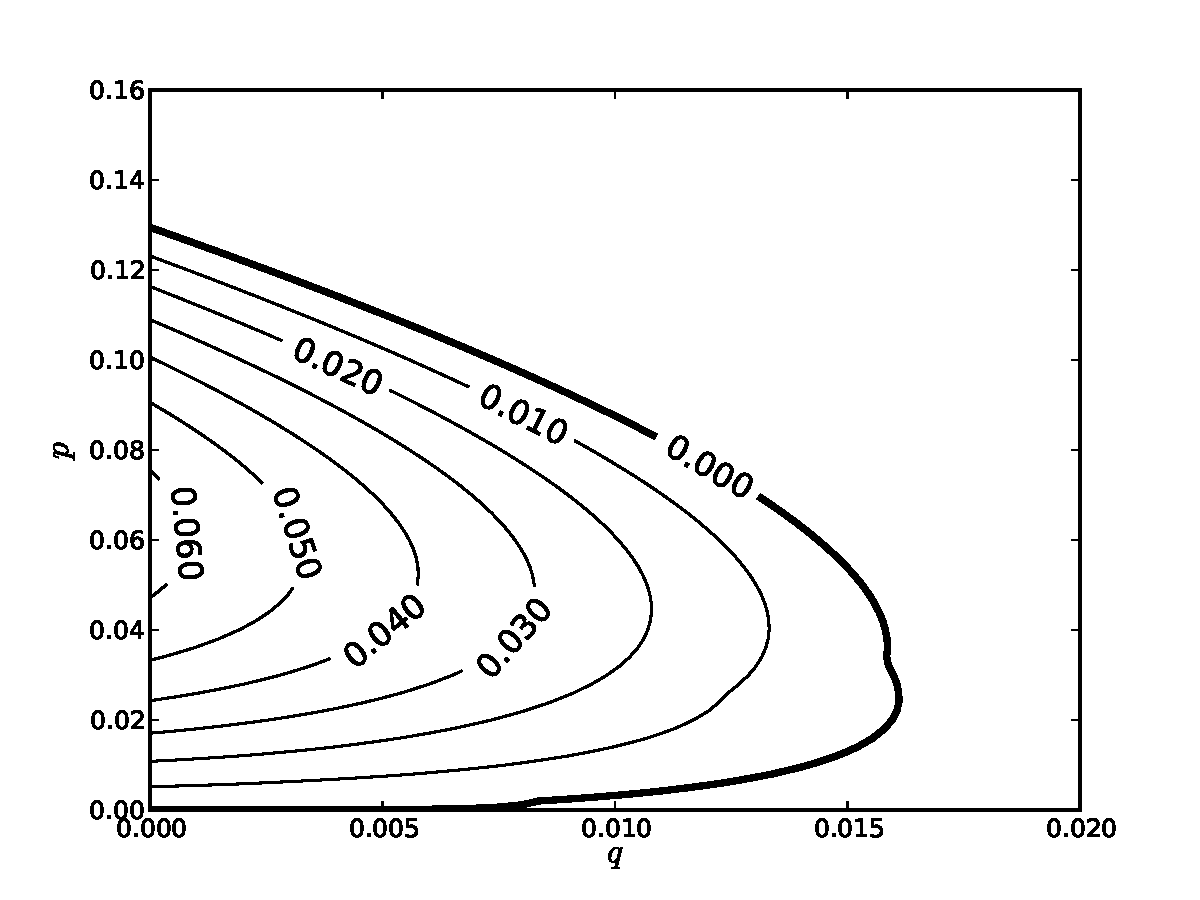
\includegraphics[width=8cm]{assets/full_lying.pdf}
  \end{center}
  \caption{Decoding success probabilities for the full quantum $6$-code with stabilser outcome mis-reporting.}
  \label{full_lying}
\end{figure}

In this case the $4$-code does not offer any encoding power over the $2$-code. The $4$-code has error-detect capacity but limited error-correct capacity, exemplified in its ability to correct isolated $X$ or $Z$ errors with probability about $0.5$. The $6$-code is the first code to offer encoding power (Fig. \ref{full_truthful}), outperforming the $2$-code for $p \le \sim 0.15$.

We looked at mis-reported stabiliser outcomes for the $6$-code (Fig. \ref{full_lying}). Due to computational constraints we were only able to find a lower bound for $p_{\text{success}}(6, p, q)$. This was obtained by modifying equation (\ref{lying_prob}) to maximise only over $a$ close to $a'$:
\begin{align} \label{approx_eq}
  P'_d= \sum_{a'\in A'} \max_{a \in N(a',x)} \left\{ \max_{l \in L} \left\{\sum_{e \in E_{a,l}} p(e) \right\} p(a' \vert a) \right\}
\end{align}
where $N(a', x) = \left\{a \in A : d(a', a) \leq x \right\}$ with $d(a', a)$ the number of stabilisers where $a'$ differs from $a$. We took $x = 2$ to produce a rough region, and then used $x=4$ to refine the boundary. The $6$-code is able to tolerate far lower stabiliser outcome mis-reporting rates, in the region of $0.5 - 1\%$.

\section{Experimental suggestion}

Our aim in this section is to provide a criterion which an experimentalist can use to verify whether a given candidate toric code set-up is providing protection.

Our criterion is based on the observation that the $2$-code is essentially equivalent to two unprotected qubits: the sydrome outcome is always $+1$ so we are unable to even detect errors and the logical operations reduce to single qubit operations. By comparing the performance of the candidate code system against that of the $2$-code we are able to say whether the candidate system is exhibiting protective power. 

We do not specify the decoder that the experimentalist must use for the larger code (decoding is trivial in the $2$-code), but in the remainder of the paper develop a provably-optimal decoder for small systems under the given error channels and use this to estimate the values of $p$ and $q$ that the experimentalist needs to obtain to satisfy the criterion. In the analysis that follows in the paper we assume that the stabiliser mis-reporting and physical qubit errors are independent events. A round of stabilisers is permitted to introduce physical qubit errors, but these must be sprinkled evenly over the lattice and not be correlated with mis-reporting sites. If strong correlations were to exist a modified decoder would give a better chance of satisfying the criterion.

We assume that an experimentalist has the ability to perform all $X$- and $Z$-stabiliser measurement operations and the logical X measurements. In a large code the logical operations are potentially tricky, given their non-local nature. Here, due to the size of the codes considered, the logical operations actually involve fewer qubits than the stabilisers, and so are likely to be less technically demanding.

Our experimental proposal is as follows:
\begin{enumerate}
  \item Measure  $X_v$, $X_h$, and the stabilisers to find intitial syndrome $a'_i$ and logical qubit states $(x^v_i, x^h_i)$\label{first_step}
  \item Wait. Manually introduce noise if required.
  \item Measure $X_v$, $X_h$, and the stabilisers to find final syndrome $a'_f$ and logical qubit states $(x^v_f, x^h_f)$
  \item Decode the calculated syndrome, $a' = a'_i \text{\,XOR\,} a'_f$, to find matching $m$ \label{decode_step}
  \item Modify $(x^v_f, x^h_f)$ to reflect what the outcomes would have been if we had applied $m$ before measurement to find $(x^v_m, x^h_m)$
  \item If $(x^v_i, x^h_i) = (x^v_m, x^h_m)$ count the round as a success; if not, count the round as a failure.\label{last_step}
  \item Repeat steps \ref{first_step} to \ref{last_step} many times to calculate an experimental successful decoding probability $P_\text{d}^\text{expt}$
\end{enumerate}

We then repeat this procedure for the $2$-code and compare the results: if the larger system outperforms the $2$-code protection is provided. 

\section{Conclusion}

We have provided a protocol and pre-computed decoder for demostrating toric encoding size at minimal scale. The $2n$-code requires a minimum of $2n^2$ physical code qubits, plus an auxiliary qubit with which we must be able to perform CNOT operations with any of the code qubits. For the $4$-code this is a requirement of $9$ qubits and for the $6$-code the requirement is $19$ qubits. The error rates provided are not unrealistic for current experimental systems. 

